% AUTO-GENERATED by code/figlib.py helpers -- do not edit
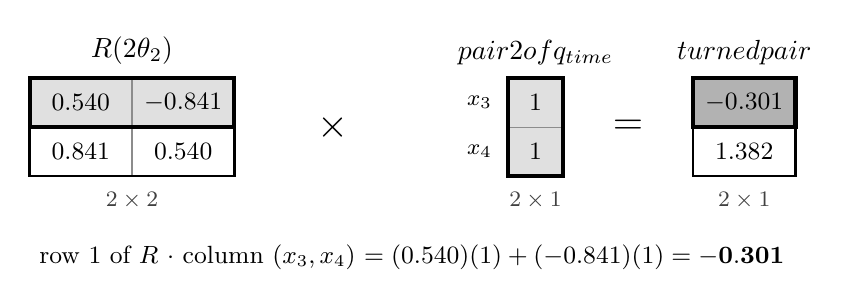
\begin{tikzpicture}
\draw[black!45, fill=black!12] (0.000,0.620) rectangle (1.300,0.000);
\node[font=\small, text=black] at (0.650,0.310) {$0.540$};
\draw[black!45, fill=black!12] (1.300,0.620) rectangle (2.600,0.000);
\node[font=\small, text=black] at (1.950,0.310) {$-0.841$};
\draw[black!45, fill=white] (0.000,0.000) rectangle (1.300,-0.620);
\node[font=\small, text=black] at (0.650,-0.310) {$0.841$};
\draw[black!45, fill=white] (1.300,0.000) rectangle (2.600,-0.620);
\node[font=\small, text=black] at (1.950,-0.310) {$0.540$};
\draw[line width=1.4pt] (0.000,0.620) rectangle (2.600,0.000);
\draw[line width=0.9pt] (0.000,0.620) rectangle (2.600,-0.620);
\node[anchor=south, font=\normalsize] at (1.300,0.670) {$R(2\theta_2)$};
\node[anchor=north, font=\footnotesize, text=black!75] at (1.300,-0.700) {$2\times2$};
\node[font=\Large] at (3.850,0) {$\times$};
\draw[black!45, fill=black!12] (6.075,0.620) rectangle (6.775,0.000);
\node[font=\small, text=black] at (6.425,0.310) {$1$};
\draw[black!45, fill=black!12] (6.075,0.000) rectangle (6.775,-0.620);
\node[font=\small, text=black] at (6.425,-0.310) {$1$};
\draw[line width=1.4pt] (6.075,0.620) rectangle (6.775,-0.620);
\draw[line width=0.9pt] (6.075,0.620) rectangle (6.775,-0.620);
\node[anchor=east, font=\footnotesize\ttfamily] at (5.995,0.310) {$x_3$};
\node[anchor=east, font=\footnotesize\ttfamily] at (5.995,-0.310) {$x_4$};
\node[anchor=south, font=\normalsize] at (6.425,0.670) {$\text{pair 2 of }\bm q_{\text{time}}$};
\node[anchor=north, font=\footnotesize, text=black!75] at (6.425,-0.700) {$2\times1$};
\node[font=\Large] at (7.600,0) {$=$};
\draw[black!45, fill=black!30] (8.425,0.620) rectangle (9.725,0.000);
\node[font=\small, text=black] at (9.075,0.310) {$-0.301$};
\draw[black!45, fill=white] (8.425,0.000) rectangle (9.725,-0.620);
\node[font=\small, text=black] at (9.075,-0.310) {$1.382$};
\draw[line width=1.6pt] (8.425,0.620) rectangle (9.725,0.000);
\draw[line width=0.9pt] (8.425,0.620) rectangle (9.725,-0.620);
\node[anchor=south, font=\normalsize] at (9.075,0.670) {$\text{turned pair}$};
\node[anchor=north, font=\footnotesize, text=black!75] at (9.075,-0.700) {$2\times1$};
\node[anchor=north west, font=\small, align=left] at (0,-1.370) {row 1 of $R$ $\cdot$ column $(x_3, x_4)$ $= (0.540)(1) + (-0.841)(1) = \mathbf{-0.301}$};
\end{tikzpicture}
